%!TEX root = ../thesis.tex
% Spellchecker ignore
% cSpell:ignore dipolpotenial, depump, acousto, levelscheme, Oshea, retroreflection, antinode, itemsep, redbluedetuning, trapdepth, giga, detuningopt, cmmnt, waals, potentialoverlap, eqref, dipolepot, wrapfigure, intensityplot, includegraphics, retroreflected, detunings, linewidth, dispersive, antinodes, pagebreak, ifpdf, graphicspath, detuned, bigskip, nano, citep, milli, detuning, medskip, mathrm
%*******************************************************************************
%****************************** First Chapter **********************************
%*******************************************************************************

\chapter{\label{chap:dipole}Theory of laser trapping of atoms}


\ifpdf{}
    \graphicspath{{Chapter1/Figs/Raster/}{Chapter1/Figs/PDF/}{Chapter1/Figs/}}
\else
    \graphicspath{{Chapter1/Figs/Vector/}{Chapter1/Figs/}}
\fi

Atoms can be trapped by a force deriving from the gradient of an optical potential 
created by the dispersive interaction of the atomic dipole moment with the intensity 
gradient of the light field. These traps can be used to confine the atoms in 3D 
and counteract gravity and confine the atoms in 3D. In the case of large detunings 
the expressions for the dipole potential and scattering rate~\cite{grimm} are 
the following:
%
\begin{align}
    U_\mathrm{dip}(z) =& \frac{3\pi c^2}{2\omega_0^3}~\frac{\Gamma}{\Delta}~I(z)~, \label{eq:dipolepot_simple}\\
    \Gamma_{\mathrm{sc}}(z) =& \frac{3\pi c^2}{2\hbar\omega_0^3}~
    {\left ( \frac{\Gamma}{\Delta} \right )}^2~I(z)~.\label{eq:scattering_simple}
\end{align}

\begin{wrapfigure}{R}{.4\textwidth}
    \centering
    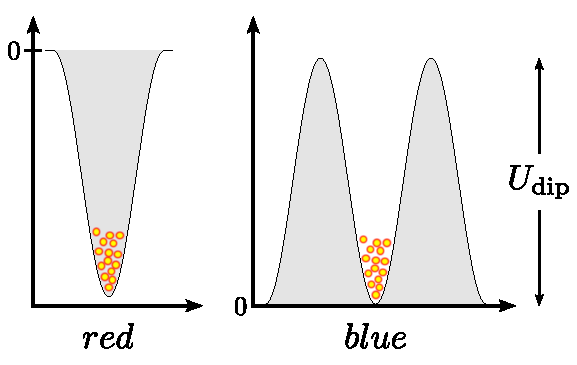
\includegraphics[width=0.35\textwidth]{redbluedetuning}    
    \caption{\label{fig:redbluedetuning} Illustration of dipole traps with red 
    and blue detuning. The grey area represents regions of high intensity.}
\end{wrapfigure}
Where \textit{c} is the speed of light, \(\Gamma \) characterizes the coupling 
rate between the two atomic levels of the atomic transition, \(\Delta \) is the 
detuning between the light and the atomic transition 
(\(\Delta = \omega - \omega_0 \)), where \(\omega \) is the driving pulsation of 
the light field, \(\omega_0 = 2\pi~\frac{c}{\lambda_0}=2\pi~\nu_0 \) the atomic 
transition pulsation and \(I(z) \) corresponds to the intensity of the light field 
at a distance \(z\) from the resonator. Dipole traps can be divided into two main 
classes, red-detuned traps (\(\Delta < 0 \)) and blue-detuned traps (\(\Delta > 0 \)). 
Below an atomic resonance (red) the dipole potential is negative and the potential 
minima are therefore found at positions of maximum intensity. For a blue-detuned 
light the potential minima correspond to minima of the intensity and the interaction 
repels atoms from the field as seen in Fig.~\ref{fig:redbluedetuning}. For our 
setup we will consider a red-detuned trap.
\pagebreak

There are three different trap configurations possible:
\begin{itemize}
    \setlength{\itemsep}{0ex}
    \item \textit{focused-beam trap}: Focused-beam traps are consisting of a 
    single strongly focused beam and have a confinement volume proportional to 
    \(z_R \times {w_0}^2 \), where \(z_R \) is the Rayleigh length and \(w_0 \) 
    is the beam waist radius.
    \item \textit{crossed-beam trap}: A crossed-beam configuration uses two beams
    of waist \(w_0\) and \(w_1\) which intersect at their foci. The confinement 
    volume reduces to the intersection of the contributing beams, which is in 
    case where \(w_0 \) is smaller than \(w_1 \): \({w_0}^2\times w_1\).
    \item \textit{standing wave trap}: In case of a standing wave trap the atoms 
    are axially confined in the antinodes of a standing wave. If the standing 
    wave is created through a retroreflection the first antinode and therefore 
    first trapping site lies at a distance of \(\frac{\lambda}{4} \) from the 
    surface (see Fig.~\ref{fig:intensityplot}). The resulting volume is in the 
    order of \({w_0}^2 \times \frac{\lambda}{4} \).
\end{itemize} 

For our experiment it is important that the atoms are as close as possible from 
the resonator, because the interacting evanescent field in the 
resonator decreases exponentially with a decay length of \(\frac{\lambda_{at} }{2\pi} \) 
where \(\lambda_{at} \) is the wavelength of the cavity field tuned to the atomic 
transition. \(5S_{1/2} \rightarrow 5P_{3/2} \) (\(D_2 \) line of Rb at 
\SI{780}{\nano\meter}) has a decay length of \SI{124}{\nano\meter}.

\begin{wrapfigure}{R}{.4\textwidth}
    \centering
    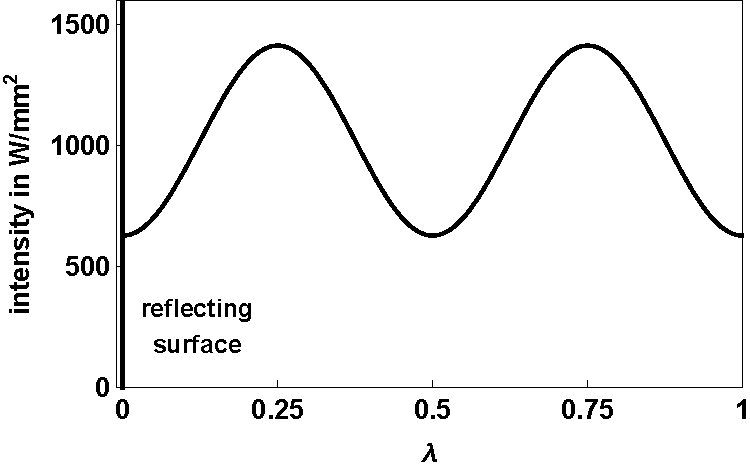
\includegraphics[width=0.35\textwidth]{intensityplot}    
    \caption{\label{fig:intensityplot} 1D Intensity distribution of a retroreflected 
    gaussian laser beam for a partial standing wave with \(r=-0.2\).}
\end{wrapfigure}
If one uses a laser closely detuned from 
the \(D_2 \) line \(5S_{1/2} \rightarrow 5P_{3/2} \) to trap the atom, i.e. 
\SI{783}{\nano\meter}, this leads to a distance of \(\frac{\lambda}{4} \approx 
\SI{190}{\nano\meter} \). This would be already too far from the resonator. 
Interestingly Rubidium atoms also have a transition from \(5S_{1/2}~\text{to}~6P_{3/2} \) 
at \SI{420}{\nano\meter} as can be seen in Fig.~\ref{fig:levelscheme}.
In the next section we will establish the trap parameters necessary to trap the
atoms.
\pagebreak

\begin{figure}[h]
    \centering
    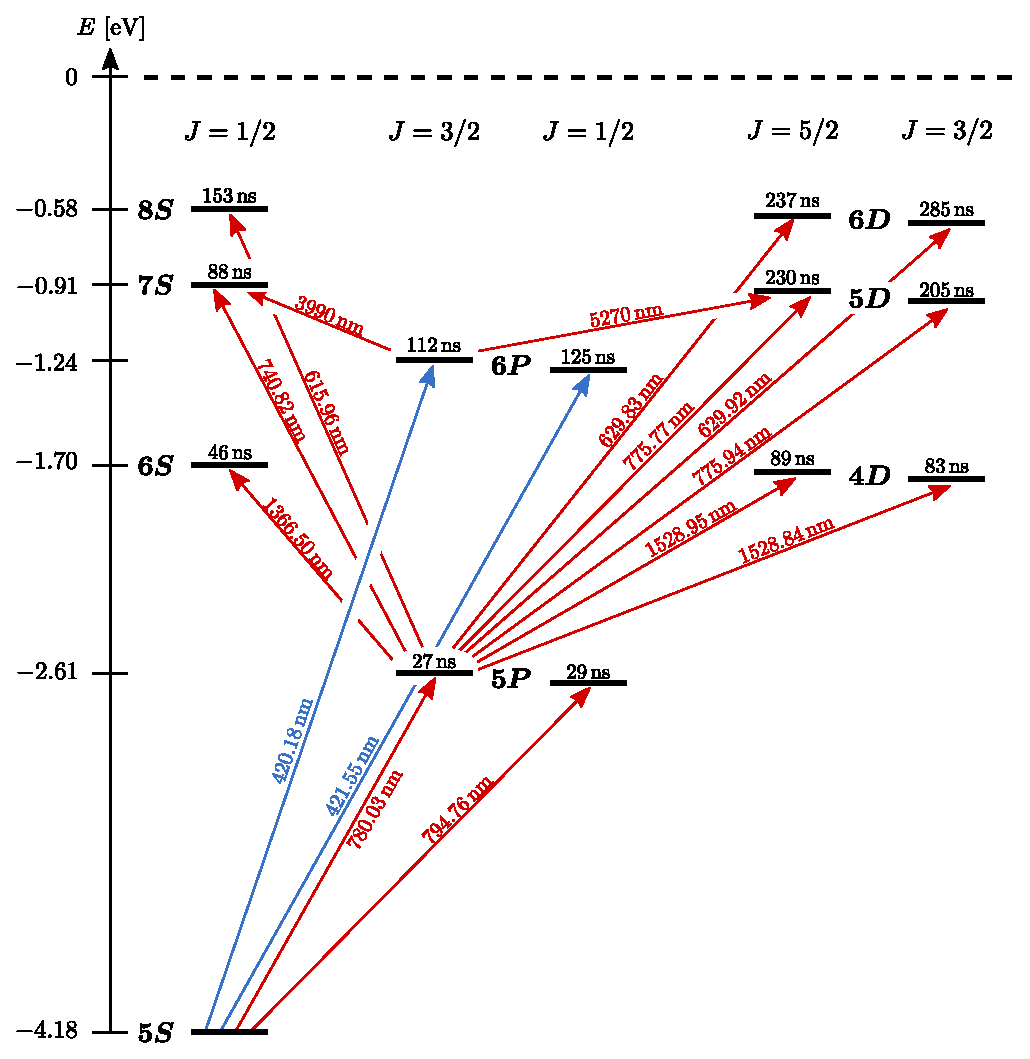
\includegraphics[width=0.9\textwidth]{levelscheme}
    \caption{\label{fig:levelscheme} Level scheme of \(^{85}\)Rb with lifetimes
    and transition wavelength of the first states~\cite{SchulzPHD}.}
\end{figure}

As we can see in Eq.~\eqref{eq:dipolepot_simple} the dipole potential is proportional 
to \(\frac{I}{\Delta} \), which means that we have two degrees of freedom, the 
detuning and the power (\(I\propto\frac{power}{cross~section} \)). To choose our 
parameters properly we have to consider some constraints. We want to keep the 
scattering rate as low as possible, because each photon scattered may depolarize 
the atom or depump the atom in which case it cannot be detected
anymore. The scattering rate is proportional 
to \(\frac{I}{\Delta^2} \) (Eq.~\ref{eq:scattering_simple}), so a detuning as big 
as possible would be beneficial. On the other hand laser power is limited 
(\(P_{\max}=\SI{80}{\milli\watt} \)), due to the maximum power output of our laser.
And additionally we do not want to send too much power onto the resonator, because 
due to the highly focused beam (\(w_0 = \SI{3.6}{\micro\meter} \)), the more
energetic wavelength and more absorption of the glass in the blue spectrum the 
resonator could be damaged. To compensate the lower laser power the detuning has 
to be small. However if \(\Delta \) smaller than the separation between the 
\(D_1 \) and \(D_2 \) lines (\SI{420}~\& \SI{421}{\nano\meter}) then we need to 
take the fine structure of the atom into account and equations~\eqref{eq:dipolepot_simple} 
and~\eqref{eq:scattering_simple} rewrite as~\cite{grimm} 
%
\begin{align}\label{eq:dipolpotenial}
    U_\mathrm{dip}(z) =& \frac{\pi c^2}{2\omega_0^3}~\left( 
        \frac{2~\Gamma_{\omega,D2}}{\Delta_{D2}} + 
        \frac{\Gamma_{\omega,D1}}{\Delta_{D1}} \right)~I(z)~, \\
    \Gamma_{\mathrm{sc}}(z) =& \frac{\pi c^2}{2\hbar\omega_0^3}~\left( 
        \frac{2~\Gamma_{\omega,D2}~\Gamma_{\omega,D2,tot} }{\Delta_{D2}^2 } + 
        \frac{\Gamma_{\omega,D1}~\Gamma_{\omega,D1,tot} }{\Delta_{D1}^2 } \right)~I(z)~.
\end{align}
%
% TODO: Add explanation of the factor of 2 in above equation and why in the 
%original equation is only one Gamma

It should be noted that as \(6P_{1/2}~\text{and}~6P_{3/2} \) are not the first
excited states, there exist several possible decay channels from there to the
ground state. \(\Gamma_{\omega,Dx} \) are the transition strengths from 
\(5S_{1/2} \rightarrow 6P_{1/2} \) and \(5S_{1/2} \rightarrow 6P_{3/2} \), while
\(\Gamma_{\omega,Dx,tot} \) represents the total decay rates of the 
\(6P_{1/2}~\text{and}~6P_{3/2} \) states with \(\frac{1}{\Gamma_{\omega,Dx,tot}} \) 
the mean lifetime of the state given in Fig.~\ref{fig:levelscheme} and \(\Delta_{Dx} \) 
represents \(\omega - \omega_{0,Dx} \). All values can be found in 
table~\ref{table:iso_prop}.

It should be noted that \(\Gamma_{6P_{3/2}}\) is 20 times weaker than 
\(\Gamma_{5P_{3/2}}\) and thus, for the same trap depth a shorter detuning or 
higher power will be needed comparatively to a dipole trap around \SI{780}{\nano\meter}.

%********************************** % First Section  **************************************
\section{Possible configuration of optical dipole trap} %Section - 1.1

\begin{figure}[h]
    \centering
    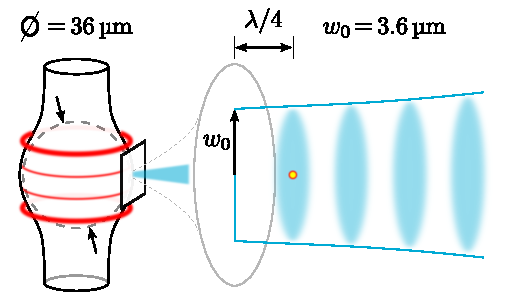
\includegraphics[width=0.6\textwidth]{resonator_trap_label}
    \caption{\label{fig:resonator_trap_label} Experimental setup and intensity 
    distribution. }
\end{figure}
To calculate the trap potential we have to derive the intensity of the standing
wave. The trap is produced by a beam focused down to at radius of \(w_0 = 
\SI{3.6}{\micro\meter} \). While the resonator diameter is \SI{36}{\micro\meter}
(as shown in Fig.~\ref{fig:resonator_trap_label}). Thus, one can consider that
the beam is retroreflected on a planar surface. With this assumption the electric 
field becomes:
\begin{align}
    \vec{E}(z) = E_0~\vec{x}~\left( e^{-i k_z z} + r e^{i k_z z} \right)
\end{align}
with \(r \) the reflection coefficient in amplitude, which is in case of a 
glass/vacuum interface \(r = -0.2 \). \(k_z \) is the wave vector in z-direction 
and equal to \(\frac{2\pi}{\lambda} \). This leads to the intensity
\begin{align}
    I(z) = \frac{ { 2| \vec{E}(z) | }^2}{\eta}
\end{align}
depicted in Fig.~\ref{fig:intensityplot}. Where 
\(\eta = \eta_0 = \frac{1}{\epsilon_0 c_0} \approx \SI{377}{\ohm} \) is the 
characteristic impedance of free space and \(\frac{2~{E_0}^2}{\eta} \) will be 
denoted as the maximum intensity \(I_0 \) and related to the power of a gaussian 
beam as
\begin{align}
    P_0 = \frac{1}{2}~I_0 {w_0}^2 \pi~.
\end{align} 
The range of power accessible is between \(0~<~P_0~<\SI{80}{\milli\watt} \), due
the maximum laser output power. 

\begin{wrapfigure}{Hr}{.4\textwidth}
    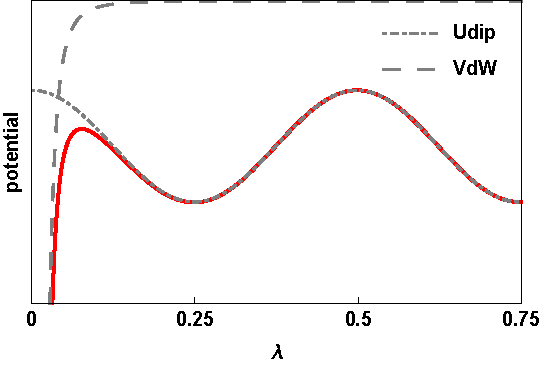
\includegraphics[width=0.35\textwidth]{potentialoverlap}    
    \caption{\label{fig:potentialoverlap} Overlap of dipole and Van-der-Waals 
    potential.}
    \vspace{2em}
    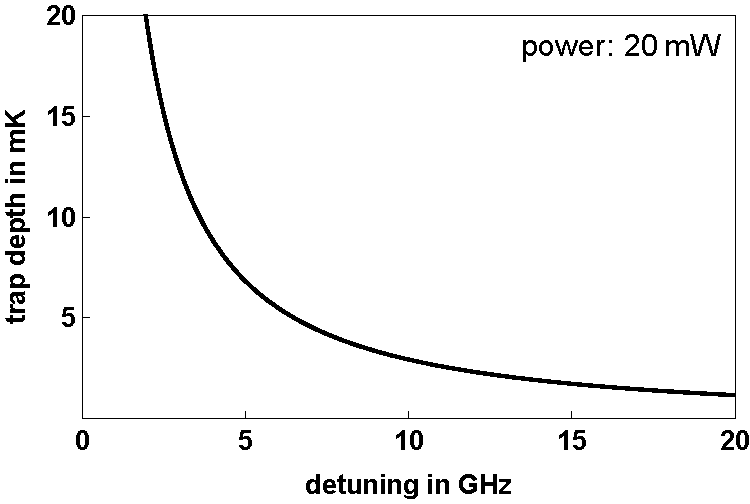
\includegraphics[width=0.35\textwidth]{detuningopt}    
    \caption{\label{fig:detuningopt} Trap depth for different detuning.}
\end{wrapfigure}

The trap depth must be bigger than the energy of the atom, here the kinetic energy 
\(E_{kin} = \frac{1}{2}m_{Rb} v^2 \) has to be taken into account due to the fact 
that the atoms are free falling for up to \SI{60}{\milli\second}. It corresponds 
in terms of temperature to \(E_{kin}/k_B = \SI{1.77}{\milli\kelvin} \). Our trap 
is conservative. When an atom is captured it gains the potential energy at its
position \(E_{pot}(z) \) and if \(E_{kin} + E_{pot}(z) \) is greater than \(E_{pot,\max}\) 
then the atom will not be trapped. Therefore one should add a safety margin to 
capture more atoms. For example a \SI{5}{\milli\kelvin} trap would capture 
\(\frac{5-1.77}{5} \approx \SI{60}{\percent} \) of atoms entering the trap if all
the atoms have the maximum kinetic energy (worst case scenario). In our setup we 
are so close to the resonator that the atoms are also sensitive to the Van-der-Waals 
potential\cite{PhysRevA.89.022511}
\begin{align}
    U_{VdW} = -\frac{C_3}{r^3}~.
\end{align} 
The \(C_3\) coefficient is \( h\cdot770\cdot10^{-18}~\si{\hertz\meter\cubed}\)
~\cite{OsheaPHD}, where \(h\) is Plank's constant.

\begin{wrapfigure}{Hr}{.4\textwidth}
    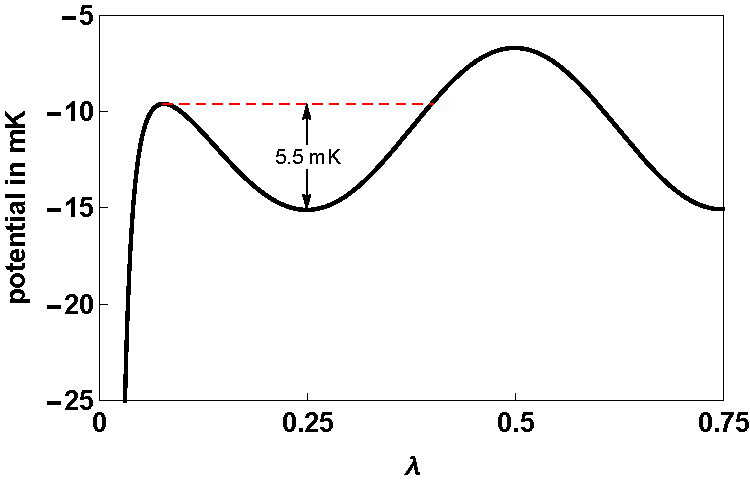
\includegraphics[width=0.35\textwidth]{trapdepth}    
    \caption{\label{fig:trapdepth} Calculated trap potential for \SI{20}{\milli\watt}
     power and a \SI{6}{\giga\hertz} detuning.}
\end{wrapfigure}

The total potential seen by the atoms is \(U_{VdW} + U_{dip} \) 
(see Fig.~\ref{fig:potentialoverlap}). The depth of the potential well is now the 
difference between the reduced first maximum and the first minimum at \(\lambda/4 \)
(see Fig.~\ref{fig:trapdepth}). 
For our trap we expect to have \SI{20}{\milli\watt} of laser power accessible. 
The power loss include locking the laser to a fixed frequency (\SI{5}{\milli\watt}), 
because the frequency deviation in free running can be on the order of 
\SI{1}{\giga\hertz} when we need to be only \SI{10}{\giga\hertz} from resonance 
away (see. Fig.~\ref{fig:detuningopt}). One also needs to take into account the 
losses due to the optical path of the beam before reaching the atoms, which will 
contain acousto-optical modulators and fiber coupling. As we can see in 
Fig.~\ref{fig:detuningopt} for \SI{20}{\milli\watt} power the detuning has to be 
lower than \SI{7}{\giga\hertz}. For a detuning of \SI{6}{\giga\hertz} we get a trap 
depth of \SI{5.5}{\milli\kelvin} as shown in Fig.~\ref{fig:trapdepth}.

In order to set the laser detuning properly, we need to realize a spectroscopy 
on the \(5S_{1/2} \rightarrow 6P_{3/2} \) transition (see Chapter 3).

As seen in equation~\ref{eq:dipolpotenial} to calculate the trap depth, the 
transition strength plays a significant role. As \(\Gamma_{6P_{3/2}}\) is harder
to determine, but can be linked to the saturation intensity by the theoretical
formula
\begin{align}
    I_{s,420} &= \frac{{\Gamma_{\omega,tot,420}}^2\cdot{\omega_{420}}^3\cdot I_{s,780}}
    {\Gamma_{\omega,420}\cdot\Gamma_{\omega,780}\cdot{\omega_{780}}^3} 
    &= \SI{126}{\watt\per\meter\squared}~,
\end{align} 
which we would like to confirm. The index 420 corresponds to 
\(5S_{1/2} \rightarrow 6P_{3/2} \) and the index 780 to 
\(5S_{1/2} \rightarrow 5P_{3/2} \). In the next chapter we will discuss how we 
can make use of the light matter interaction to measure \(I_s\) by realising an 
absorption spectroscopy measurement.

